\documentclass{article}
\usepackage[utf8]{inputenc}
\usepackage[polish]{babel}
\usepackage[T1]{fontenc}
\usepackage{hyperref}
\usepackage{amsmath}
\usepackage{float}
\usepackage{pifont}
\usepackage{capt-of}
\usepackage{graphicx} % Required for inserting images

\title{Zanieczyszczenia powietrza we Wrocławiu - analiza modelem ARMA}
\author{Patrycja Nowicka, Gabriela Karaś}
\date{}
\begin{document}

\maketitle

\section{Wstęp oraz informacje o danych}
Celem niniejszej pracy jest przeprowadzenie analizy szeregów czasowych dotyczących godzinowych pomiarów stężenia pyłu zawieszonego PM2.5 we Wrocławiu, z wykorzystaniem modeli ARMA. Praca ma na celu identyfikację struktury czasowej, ocenę stacjonarności i sezonowości danych, a także budowę modelu prognozującego krótkoterminowe zmiany stężenia PM2.5. Uzyskane wyniki mają służyć lepszemu zrozumieniu dynamiki zanieczyszczenia powietrza. \\

Wybrane dane dotyczą zanieczyszczeń powietrza pyłem zawieszonym PM2.5. Pomiary zostały wykonane w ramach projektu Grow Green, w okresie od 1.09.2018 do 31.09.2019. Pomiar jakości powietrza następował codziennie, co godzinę, w stacji Wojewódzkiego Inspektoratu Ochrony Środowiska  przy ul. Conrada-Korzeniowskiego 18 we Wrocławiu. Baza danych zawiera 8736 rekordów w dwóch kolumnach, gdzie w pierwszej kolumnie jest data oraz godzina pomiaru, a w drugiej znajduje się pomiar stężenia pyłu zawieszonego PM2.5, w jednostce $\frac{\mu g}{m^3}$. \\

Dane można znaleźć pod następującym odnośnikiem: 
\href{https://www.wroclaw.pl/open-data/dataset/grow-green-jakosc-powietrza-monitoring-wstepny-i-koncowy/resource/3bc61a00-4570-4201-9c34-fcde2067f36e}{Jakość powietrza}.
\\

\begin{center}
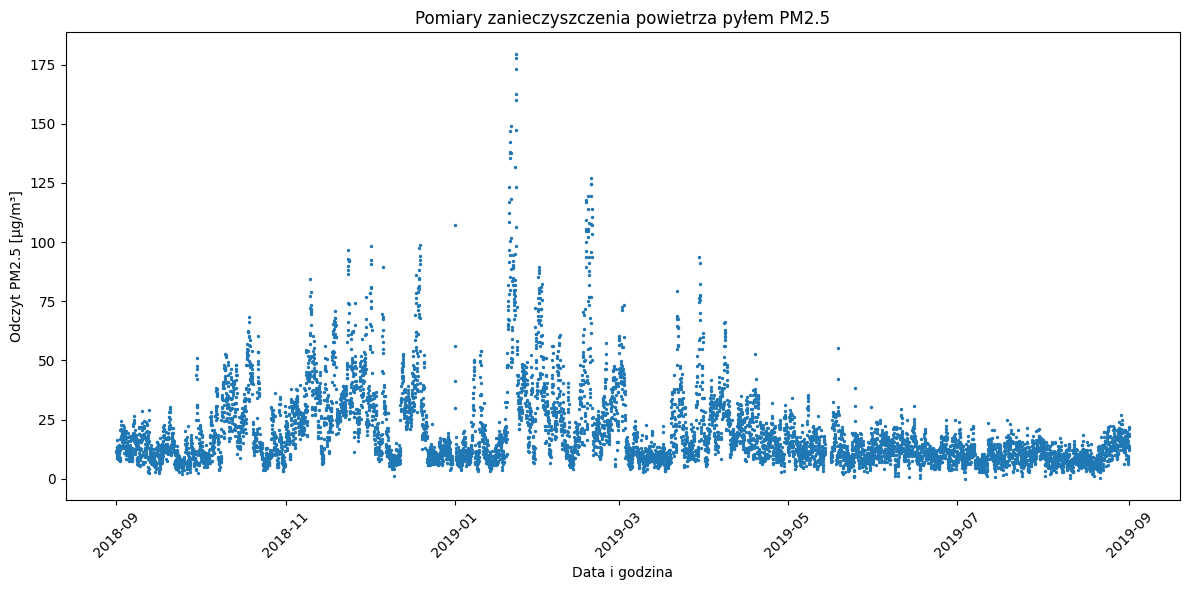
\includegraphics[width=0.85\linewidth]{output.png}
  \vspace{0.5em} % odstęp między obrazkiem a podpisem
  \\
  {\small \textbf{Rysunek 1.} Wizualizacja danych}
\end{center}

\section{Przygotowanie danych do analizy}
\subsection{Braki danych i wartości nieprawidłowe}
Przygotowanie rozpoczęło się od identyfikacji, czy w zbiorze znajdują się braki danych. 
\begin{table}[h]
\centering
    \caption{Liczba rekordów w zbiorze danych}
    \begin{tabular}{|c|c|}
    \hline
    Przed usunięciem braków danych & 8736 \\
    \hline
    Po usunięciu braków danych & 8640 \\
    \hline
    \end{tabular}
\end{table} \\
Widać zatem, że 96 razy pomiar nie został zarejestrowany. \\
Zbadane zostały też wartości, czy mieszczą się w rozsądnym przedziale. 
\begin{table}[h]
    \centering
    \caption{Wartości ekstremalne zbioru danych}
    \begin{tabular}{|c|c|}
    \hline
    \textbf{Wartość} & \textbf{Wielkość} \\
    \hline
    Minimum & 0.0 \\
    Maksimum & 179.7 \\
    \hline
    \end{tabular}
\end{table} \\
Nie występują wartości ujemne, które byłyby nieprawidłowe w naszym przypadku, wartość maksymalna również nie jest bardzo wysoka, mieści się ona w realistycznych granicach pomiaru jakości powietrza. 

\subsection{Funkcja autokowariancji oraz częściowej autokowariancji}

\begin{center}
  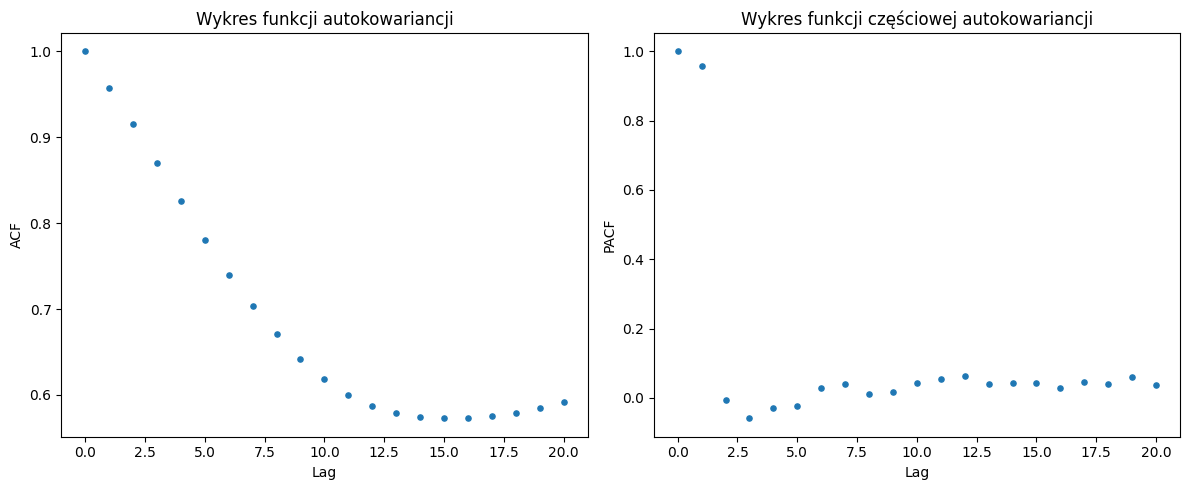
\includegraphics[width=\linewidth]{output2.png}

  \vspace{0.5em} % odstęp między obrazkiem a podpisem
    \\
  {\small \textbf{Rysunek 2.} Funkcje ACF i PACF}
\end{center}

Analiza wykresów ACF oraz PACF pozwala na wyciągnięcie następujących wniosków dotyczących struktury badanego szeregu czasowego.
Wykres autokorelacji (ACF) wykazuje bardzo powolny, niemal liniowy spadek wartości. Nawet przy lagu 20 autokorelacja pozostaje na wysokim poziomie (powyżej 0.5). Jest to klasyczny sygnał świadczący o niestacjonarności szeregu lub występowaniu bardzo silnego trendu.
Na wykresie autokorelacji częściowej (PACF) widoczne jest jedno wyraźne, dominujące „szarpnięcie” dla pierwszego opóźnienia ($lag=1$), po którym następuje gwałtowny spadek wartości w okolicę zera. Sugeruje to, że proces ma silny komponent autoregresyjny rzędu pierwszego – AR(1).
Ze względu na fakt, że ACF nie wygasza się szybko do zera (co jest wymogiem dla procesów stacjonarnych), potwierdzona zostaje konieczność zastosowania różnicowania w celu sprowadzenia szeregu do postaci stacjonarnej przed dalszą identyfikacją modelu ARMA.

\subsection{Test ADF}
Przeprowadzimy teraz test ADF (Augmented Dickey-Fuller Test), żeby sprawdzić czy wybrane dane są stacjonarne. 
\paragraph{Teoria}
Test ADF polega na testowaniu następujących hipotez: 

\[
\begin{cases}
H_0: \text{szereg ma jednostkowy pierwiastek (jest niestacjonarny)} \\
H_1: \text{szereg jest stacjonarny}
\end{cases}
\]

Model regresji, na którym opiera się test ADF, ma postać:

\[
\Delta y_t = \alpha + \beta t + \gamma y_{t-1} + \sum_{i=1}^p \delta_i \Delta y_{t-i} + \varepsilon_t,
\]

gdzie:

\begin{itemize}
    \item \( y_t \) --- wartość szeregu czasowego w chwili \( t \),
    \item \( \Delta y_t = y_t - y_{t-1} \) --- pierwsza różnica szeregu,
    \item \( \alpha \) --- wyraz wolny (stała),
    \item \( \beta t \) --- trend liniowy (opcjonalny),
    \item \( \gamma \) --- parametr testowany, odpowiedzialny za obecność jednostkowego pierwiastka,
    \item \( \delta_i \) --- współczynniki przy opóźnieniach różnicowanych wartości,
    \item \( p \) --- liczba opóźnień dołączonych do modelu,
    \item \( \varepsilon_t \) --- składnik losowy (biały szum).
\end{itemize}

Interpretacja wyniku testu opiera się na wartości statystyki testowej:

\[
\tau = \frac{\hat{\gamma}}{\mathrm{SE}(\hat{\gamma})},
\]

gdzie \( \hat{\gamma} \) to estymator parametru \( \gamma \), a \( \mathrm{SE}(\hat{\gamma}) \) to jego błąd standardowy.

\[
\left\{
\begin{array}{l}
H_0: \gamma = 0 \quad \text{(obecność jednostkowego pierwiastka, niestacjonarność szeregu)} \\
H_1: \gamma < 0 \quad \text{(szereg jest stacjonarny)}
\end{array}
\right.
\]
 
\paragraph{Wyniki modelu}
Dla wybranych danych mamy natępujące wartości:
\begin{table}[h]
\centering
\caption{Test ADF dla poziomu istotności $\alpha = 0.05$}
    \begin{tabular}{|c|c|}
    \hline
    P-wartość & $2.23 \cdot 10^{-10}$ \\
    \hline
    Wartość statystyki ADF & $-7.21$ \\
    \hline
    \end{tabular}
\end{table} \\
Widzimy że p-wartość jest dużo niższa od poziomu istotności, zatem odrzucamy hipotezę o stacjonarności danych. 

\subsection{Transformacja Boxa-Coxa}
Kolejnym krokiem będzie sprawdzenie, czy wariancja jest stabilna. Jeśli jest niestabilna, warto jest zastosować transformację Boxa-Coxa, aby ją ustabilizować. \\

\begin{center}
  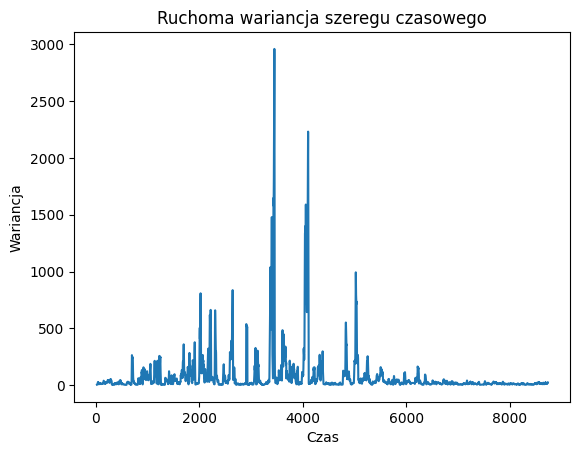
\includegraphics[width=0.8\linewidth]{output3.png}

  \vspace{0.5em} % odstęp między obrazkiem a podpisem
\\
  {\small \textbf{Rysunek 3.} Wykres wariancji}
\end{center}
Ruchoma wariancja jest bardzo niestabilna, oznacza to silną heteroskedastyczność. W takiej sytuacji transformacja stabilizująca wariancję jest potrzebna. Zatem wykorzystamy teraz transformatę Boxa-Coxa. 

\paragraph{Teoria}
Transformatę Boxa-Coxa definiuje się następująco: \\

\[
y^{(\lambda)} =
\begin{cases}
\dfrac{y^\lambda - 1}{\lambda}, & \lambda \neq 0, \\[10pt]
\ln(y), & \lambda = 0,
\end{cases}
\]

gdzie:

\begin{itemize}
    \item \( y > 0 \) — oryginalne dane (dodatnie),
    \item \( \lambda \in \mathbb{R} \) — parametr transformacji,
    \item \( y^{(\lambda)} \) — przetransformowana zmienna.
\end{itemize} \\

Aby skorzystać z tego wzoru, parametr \(\lambda\) dobiera się tak, aby zmaksymalizować logarytm funkcji wiarygodności dla przetransformowanych danych:

\[
\ell(\lambda) = -\frac{n}{2} \log \left( \frac{1}{n} \sum_{t=1}^n \left(y_t^{(\lambda)} - \bar{y}^{(\lambda)} \right)^2 \right) + (\lambda - 1) \sum_{t=1}^n \log y_t,
\]

gdzie:

\begin{itemize}
    \item \( n \) — liczba obserwacji,  
    \item  \( \bar{y}^{(\lambda)} \) — średnia przetransformowanych danych.
\end{itemize}

\paragraph{Wyniki modelu}
Dla wybranych danych, parametr transformacji modelu \(\lambda\) jest równy \fbox{$\lambda = -0.20$}, a przetransformowane dane wyglądają następująco:

\begin{center}
  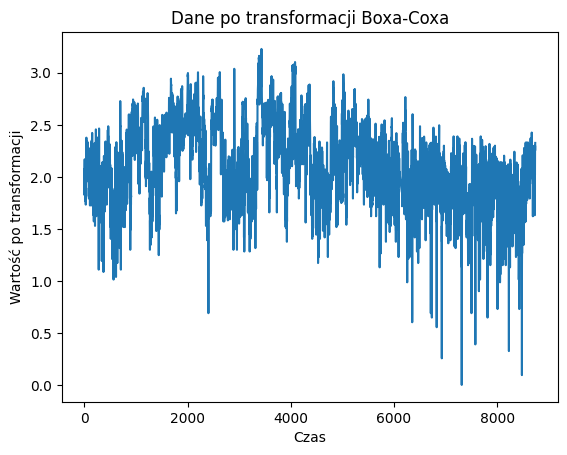
\includegraphics[width=0.8\linewidth]{output44.png}

  \vspace{0.5em} % odstęp między obrazkiem a podpisem

  {\small \textbf{Rysunek 4.} Przetransformowane dane}
\end{center}
Dane są już ustabilizowane, więc można przejść teraz do trendów deterministycznych. 

\subsection{Oczyszczenie danych z trendów deterministycznych}
\paragraph{Teoria}
\ding{172} Różnicowanie to popularna metoda stosowana w analizie szeregów czasowych w celu usunięcia niestacjonarności, szczególnie trendu i sezonowości. \\

Różnicowanie zwykłe polega na obliczeniu różnicy między kolejnymi obserwacjami szeregu czasowego:

\[
\nabla y_t = y_t - y_{t-1},
\]

gdzie:

\begin{itemize}
    \item \( y_t \) — wartość szeregu w chwili \( t \),
    \item \( \nabla y_t \) — pierwsza różnica (różnicowanie pierwszego rzędu).
\end{itemize}

Różnicowanie może być wykonywane wielokrotnie (różnicowanie rzędu \( d \)):

\[
\nabla^d y_t = \nabla^{d-1} y_t - \nabla^{d-1} y_{t-1}.
\]

Celem jest uzyskanie szeregu stacjonarnego, eliminując trend. \\

\ding{173} Różnicowanie sezonowe usuwa sezonowość o okresie \( s \) (np. \( s=12 \) dla danych miesięcznych):

\[
\nabla_s y_t = y_t - y_{t-s}.
\]

Można również stosować różnicowanie sezonowe wielokrotne (rzędu \( D \)):

\[
\nabla_s^D y_t = \nabla_s^{D-1} y_t - \nabla_s^{D-1} y_{t-s}.
\] 

\paragraph{Wyniki modelu} Dla wybranych danych zostały przetestowane obydwa rodzaje różnicowania. 

\begin{center}
  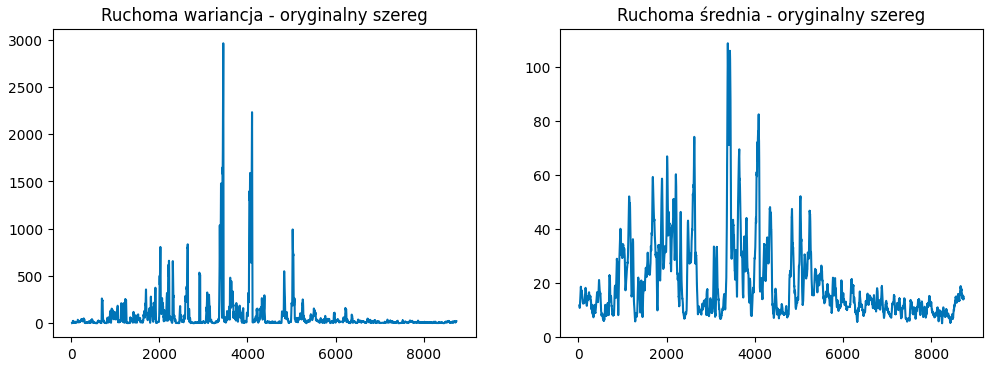
\includegraphics[width=0.9\linewidth]{output5.png}

  \vspace{0.5em} % odstęp między obrazkiem a podpisem

  {\small \textbf{Rysunek 5.} Wykres wariancji oraz wykres średniej}
\end{center}

Statystyki ruchome dla oryginalnego szeregu:
\begin{itemize}
    \item średnia wariancja - 78.4014
    \item średnia średnia - 19.6117
\end{itemize} 

\begin{center}
  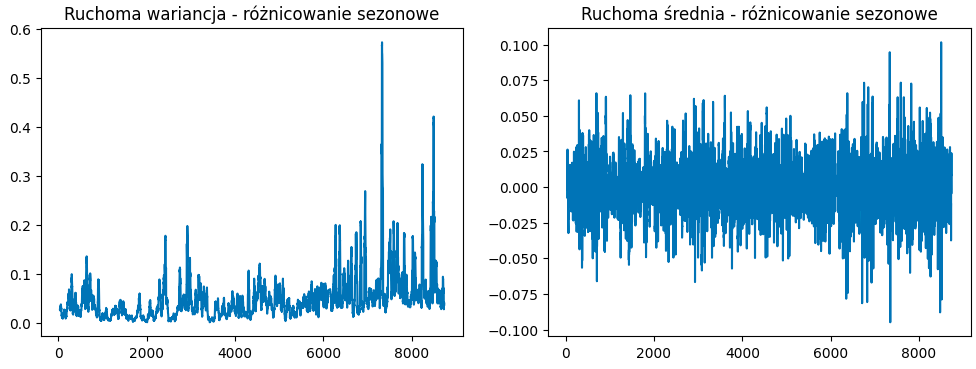
\includegraphics[width=0.9\linewidth]{output6.png}

  \vspace{0.5em} % odstęp między obrazkiem a podpisem

  {\small \textbf{Rysunek 6.} Wykres wariancji oraz wykres średniej}
\end{center}
Statystyki ruchome dla różnicowania sezonowego: 
\begin{itemize}
    \item średnia wariancja - 0.0508
    \item średnia średnia - 0.000
\end{itemize}

\begin{center}
  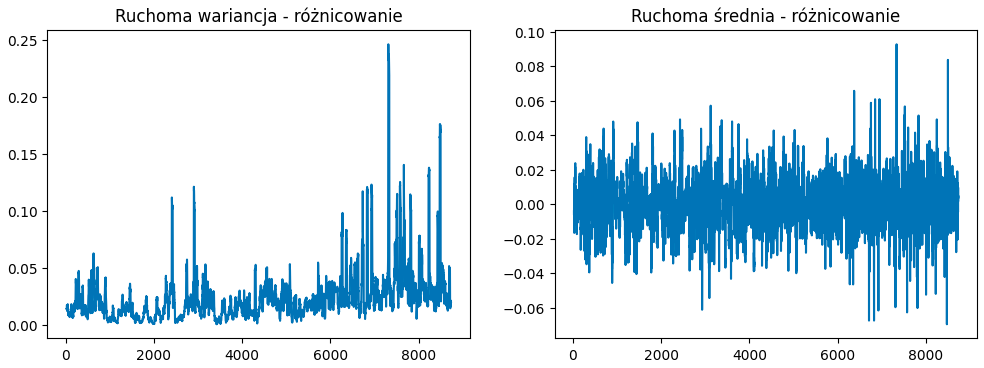
\includegraphics[width=0.9\linewidth]{output7.png}

  \vspace{0.5em} % odstęp między obrazkiem a podpisem

  {\small \textbf{Rysunek 7.} Wykres wariancji oraz wykres średniej}
\end{center}
Statystyki ruchome dla różnicowania: 
\begin{itemize}
    \item średnia wariancja - 0.0248
    \item średnia średnia 0.000
\end{itemize} 

Wstępna analiza surowego szeregu stężeń PM2.5 wykazała silną heteroskedastyczność (zmienność wariancji w czasie) oraz niestacjonarność średniej. Ruchoma wariancja była bardzo wysoka (średnio 78.40), a wykresy wskazywały na liczne wartości odstające i piki zanieczyszczeń. Zastosowanie transformacji Boxa-Coxa oraz różnicowania pozwoliło na drastyczną stabilizację parametrów. Średnia wariancja spadła do poziomu 0.0248, a ruchoma średnia oscyluje wokół zera (0.0000). Szereg po przekształceniach charakteryzuje się stałymi momentami statystycznymi.

\subsection{Funkcja autokowariancji oraz częściowej autokowariancji dla uzyskanego szeregu}

\begin{center}
  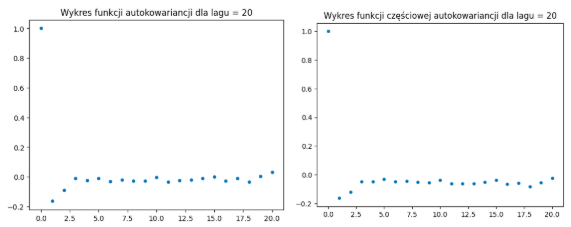
\includegraphics[width=0.9\linewidth]{output8.png}

  \vspace{0.5em} % odstęp między obrazkiem a podpisem

  {\small \textbf{Rysunek 8.} Wykresy ACF i PACF}
\end{center}
Zastosowanie operatora różnicowania zwykłego fundamentalnie zmieniło strukturę korelacyjną szeregu. W przeciwieństwie do szeregu surowego, funkcja ACF gwałtownie wygasa do zera już po pierwszych opóźnieniach. Jest to empiryczny dowód na skuteczne usunięcie trendu i sprowadzenie procesu do postaci stacjonarnej. Na wykresie PACF nadal widoczne jest istotne statystycznie opóźnienie dla $lag=1$.

\subsection{Test ADF dla uzyskanego szeregu}
Przeprowadzimy ponownie test ADF (Augmented Dickey-Fuller Test), żeby sprawdzić czy wybrane dane są stacjonarne. 

\begin{table}[h]
\centering
\caption{Test ADF}
    \begin{tabular}{|c|c|}
    \hline
    P-wartość & $0.000$ \\
    \hline
    Wartość statystyki ADF & $-20.1269$ \\
    \hline
    Krytyczna wartość 1\% & $-3.4211$ \\
    \hline
    Krytyczna wartość 5\% & $-2.8619$ \\
    \hline
    Krytyczna wartość 10\% & $-2.5669$ \\
    \hline
    \end{tabular}
\end{table} \\

Uzyskana wartość statystyki testowej ($-20,1269$) jest istotnie niższa od wszystkich wartości krytycznych, w tym dla najbardziej rygorystycznego poziomu istotności $1\%$. Ponadto, p-wartość bliska zeru pozwala na jednoznaczne odrzucenie hipotezy zerowej o niestacjonarności na rzecz hipotezy alternatywnej. Ostatecznie proces po różnicowaniu jest stacjonarny w sensie słabym.

\section{Modelowanie danych przy pomocy ARMA}
\subsection{Dobranie rzędu modelu}
Użyjemy modelu hybrydowego ARMA(3,1)+GARCH(1,1) z rozkładem t-Studenta dla szumu. Pozwala on na jednoczesne modelowanie średniej (część ARMA) oraz warunkowej wariancji (część GARCH). \\
Równanie średniej (ARMA(3,1)):$$y_t = \phi_0 + \sum_{i=1}^3 \phi_i y_{t-i} + \theta_1 \varepsilon_{t-1} + \varepsilon_t$$ \\
gdzie:

\begin{itemize}
    \item $y_t$ - wartość stężenia PM2.5 (po transformacji) w czasie $t$,
    \item $\phi_0$ - wyraz wolny modelu średniej,
    \item $\phi_1, \phi_2,\phi_3$ - parametry autoregresyjne, określające wpływ wartości zanieczyszczeń z poprzednich trzech godzin na godzinę bieżącą,
    \item $\theta_1$ - parametr średniej ruchomej, opisujący wpływ błędu prognozy z godziny poprzedniej,
    \item $\varepsilon_t$ - składnik losowy w czasie $t$, reprezentujący nieprzewidziane szoki (np. nagła zmiana pogody) 
\end{itemize}

Równanie wariancji (GARCH(1,1)):$$\sigma_t^2 = \omega + \alpha \varepsilon_{t-1}^2 + \beta \sigma_{t-1}^2$$ \\
gdzie:

\begin{itemize}
    \item $\sigma_t^2$ -  wariancja warunkowa (zmienność) w czasie $t$. Jest to miara niepewności lub ryzyka wystąpienia skoków zanieczyszczeń,
    \item $\omega$ - stała w równaniu wariancji (musi być $> 0$), wyznaczająca długookresowy poziom zmienności,
    \item $\alpha$ - parametr ARCH. Mierzy reakcję wariancji na nagłe szoki. Wysoka wartość $\alpha$ oznacza, że system gwałtownie reaguje na piki zanieczyszczeń,
    \item $\beta$ - parametr GARCH. Odpowiada za "pamięć" wariancji. Wysoka wartość $\beta$ oznacza, że okresy wysokiej zmienności utrzymują się długo (efekt skupisk zmienności),
    \item $\alpha + \beta$ - suma tych parametrów określa trwałość zmienności. Wartość bliska $1$ sugeruje, że skutki ataku smogu wygasają bardzo powolnie.
\end{itemize}

Dla rozkładu szumu zastosujemy rozkład t-Studenta, aby uwzględnić występowanie wartości ekstremalnych w pomiarach PM2.5. \\

W celu oceny jakości dopasowania modelu oraz porównania go z alternatywnymi specyfikacjami, posłużono się logarytmem funkcji wiarygodności (Log-Likelihood) oraz kryteriami informacyjnymi:
\begin{itemize}
\item \textbf{AIC (Akaike Information Criterion):} $AIC = -2L + 2k$
\item \textbf{BIC (Bayesian Information Criterion):} $BIC = -2L + k \ln(n)$
\end{itemize}g
dzie $L$ to wartość funkcji wiarygodności, $k$ to liczba parametrów, a $n$ to liczba obserwacji. Szukamy modelu, dla którego wartości AIC i BIC są najniższe. \\

Przeprowadziliśmy testy jakości dopasowania modelu do danych dla różnych wartości parametrów $p, q, \alpha, \beta$ dla modelu ARMA($p,q$)+GARCH($\alpha, \beta$). Na podstawie przeprowadzonych obliczeń wybraliśmy model ARMA(3,1)+GARCH(1,1) jako najlepiej dopasowany. Wyniki analizy dla tego modelu są następujące:
\begin{enumerate}
\item \textbf{Istotność parametrów:} W modelu średniej (ARMA) wszystkie parametry autoregresyjne ($\phi_1, \phi_2, \phi_3$) oraz parametr średniej ruchomej ($\theta_1$) posiadają wartości $P>|z|$ równe $0.000$. Oznacza to, że są one statystycznie istotne na bardzo wysokim poziomie ufności.
\item \textbf{Parametry zmienności (GARCH):}
\begin{itemize}
\item Parametr $\alpha$ (ARCH) wynosi ok. $0.1666$, co oznacza umiarkowaną reakcję na nagłe szoki.
\item Parametr $\beta$ (GARCH) wynosi ok. $0.7856$, co wskazuje na silną "pamięć" zmienności.
\item Suma $\alpha + \beta \approx 0.952$. Wartość ta jest bliska jedności, co potwierdza, że skutki szoków zanieczyszczeń wygasają powoli, a okresy wysokiego smogu mają tendencję do długotrwałego utrzymywania się.
\end{itemize}
\item \textbf{Rozkład t-Studenta:} Wyestymowany parametr liczby stopni swobody ($\nu$) wynosi ok. $6.01$. Niska wartość tego parametru (poniżej 10) potwierdza słuszność użycia rozkładu t-Studenta – dane o PM2.5 charakteryzują się "grubymi ogonami", czyli częstym występowaniem wartości ekstremalnych.
\item \textbf{Kryteria informacyjne:} Model uzyskał bardzo niskie wartości kryteriów: $AIC = -10172.2$ oraz $BIC = -10143.9$. Tak niskie (ujemne) wartości w porównaniu do prostszych modeli bazowych świadczą o bardzo dobrym dopasowaniu modelu do danych godzinowych. Za to dla wartości Log-Likelihood = 5090.08, jako że jest tu użyta metoda największej wiarygodności, wysoki wynik też oznacza dobre dopasowanie do danych. 
\end{enumerate}


\begin{table}[h!]
\centering
\caption{Statystyki dopasowania i kryteria informacyjne}
\label{tab:kryteria}
\begin{tabular}{|l|r|}
\hline
\textbf{Kryterium / Statystyka} & \textbf{Wartość} \\ \hline
Log-Likelihood & 5090.08 \\ \hline
AIC & -10172.2 \\ \hline
BIC & -10143.9 \\ \hline
Suma $\alpha + \beta$ & 0.9522 \\ \hline
Prob(Q) Ljung-Box & 0.95 \\ \hline
\end{tabular}
\end{table}

\subsection{Estymacja parametrów modelu wybraną metodą}

\begin{table}[h!]
\centering
\caption{Wyniki estymacji modelu hybrydowego dla danych PM2.5}
\label{tab:wyniki_modelu}
\begin{tabular}{lcccc}
\hline
\textbf{Parametr} & \textbf{Symbol} & \textbf{Współczynnik} & \textbf{Std. Error} & \textbf{P-value} \\ \hline
\multicolumn{5}{l}{\textbf{Model Średniej (ARIMA 3,0,1)}} \\
Lag 1 (AR) & $\phi_1$ & 0,7429 & 0,008 & 0,000 \\
Lag 2 (AR) & $\phi_2$ & 0,0402 & 0,011 & 0,000 \\
Lag 3 (AR) & $\phi_3$ & 0,0510 & 0,010 & 0,000 \\
Lag 1 (MA) & $\theta_1$ & -0,9733 & 0,004 & 0,000 \\ \hline
\multicolumn{5}{l}{\textbf{Model Wariancji (GARCH 1,1)}} \\
Stała & $\omega$ & 0,0013 & 0,002 & 0,630 \\
ARCH & $\alpha_1$ & 0,1666 & 0,156 & 0,286 \\
GARCH & $\beta_1$ & 0,7856 & 0,267 & 0,003 \\ \hline
\multicolumn{5}{l}{\textbf{Rozkład (t-Student)}} \\
Stopnie swobody & $\nu$ & 6,0127 & 0,418 & 0,000 \\ \hline
\end{tabular}
\end{table}

\paragraph{Analiza tabeli:}
\textbf{Dla ARIMA:} Wszystkie parametry autoregresyjne ($\phi_1, \phi_2, \phi_3$) oraz średniej ruchomej ($\theta_1$) są wysoce istotne statystycznie ($p < 0,05$). Bardzo wysoki współczynnik dla pierwszego opóźnienia ($0,7429$) potwierdza, że dzisiejszy poziom zanieczyszczeń jest silnie skorelowany z dniem wczorajszym. Model poprawnie wychwytuje inercję smogu we Wrocławiu. \\
\textbf{Dla GARCH:} Parametr $\beta_1 = 0,7856$ jest statystycznie istotny ($p = 0,003$). Oznacza to, że proces wariancji ma "pamięć", wysoka zmienność (niestabilność smogu) ma tendencję do utrzymywania się przez dłuższy czas. Suma $\alpha + \beta$ wynosi około $0,9522$. Jest to wartość bliska jedności, co wskazuje na bardzo dużą persystencję szumów. Oznacza to, że jeśli wystąpi nagły skok zanieczyszczenia, system będzie potrzebował wielu dni, aby wrócić do stanu równowagi.\\
\textbf{Dla t-Student:} Parametr $\nu$ wynosi 6,01. Wartość ta jest niska (standardowy rozkład normalny ma $\nu = \infty$), potwierdza to występowanie tzw. grubych ogonów.
Ekstremalne wartości smogu (piki zagrażające zdrowiu) pojawiają się znacznie częściej, niż przewidywałby to rozkład normalny. \\

\begin{center}
  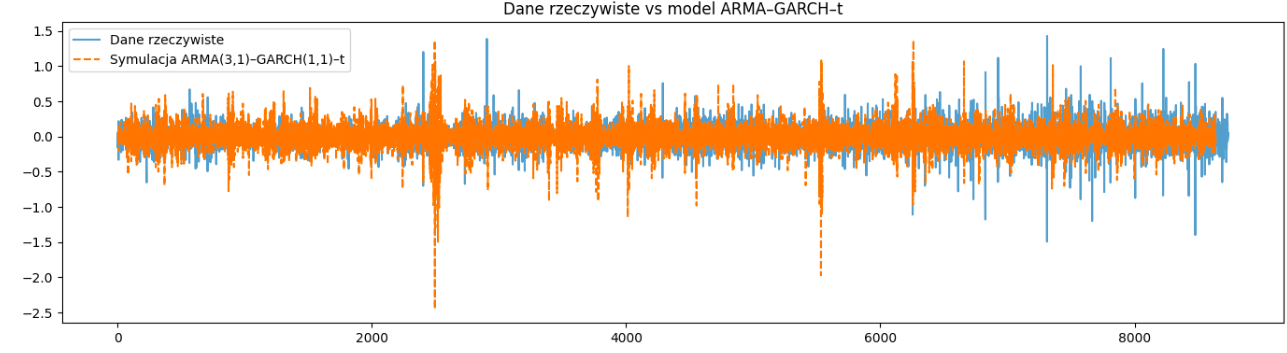
\includegraphics[width=\linewidth]{output9.png}

  \vspace{0.5em} % odstęp między obrazkiem a podpisem

  {\small \textbf{Rysunek 9.} Porównanie danych rzeczywistych z trajektorią symulowaną przy użyciu modelu ARMA(3,1)+GARCH(1,1)-t}
\end{center}

Porównanie danych rzeczywistych z wartościami dopasowanymi przez model ARMA(3,1)+GARCH(1,1) wykazuje bardzo wysoką zbieżność. Model precyzyjnie śledzi dynamikę zmian stężeń PM2.5, poprawnie reagując na nagłe piki zanieczyszczeń. Zastosowanie rozkładu t-Studenta pozwoliło na lepsze dopasowanie w obszarach wartości ekstremalnych, które w przypadku smogu mają kluczowe znaczenie.
\section{Ocena dopasowania modelu}
\subsection{Przedziały ufności dla PACF/ACF}
Kluczowym etapem weryfikacji poprawności dopasowania modelu klasy ARMA-GARCH jest analiza jego reszt standaryzowanych. Celem tej procedury jest sprawdzenie, czy model zdołał wyodrębnić z szeregu czasowego PM2.5 wszystkie istotne zależności statystyczne.\\
W idealnie dopasowanym modelu reszty powinny przyjąć formę tzw. szumu białego, czyli procesu, w którym wartości błędu w poszczególnych momentach czasu są od siebie niezależne. Do weryfikacji tej hipotezy wykorzystuje się korelagramy funkcji autokorelacji (ACF) oraz autokorelacji cząstkowej (PACF).\\
Podstawowym narzędziem diagnostycznym na poniższych wykresach są przedziały ufności (zaznaczone kolorem niebieskim), wyznaczone dla poziomu istotności $\alpha = 0,05$. Przedziały te definiują obszar, w którym korelacja jest uznawana za nieistotną statystycznie.
\begin{itemize}
    \item Jeśli słupki autokorelacji mieszczą się wewnątrz tych granic, oznacza to, że błędy modelu są losowe,
    \item Występowanie słupków poza tym obszarem sugeruje, że model nie uwzględnił pewnych cyklicznych lub systematycznych zależności występujących w danych o jakości powietrza we Wrocławiu.
\end{itemize}

\begin{center}
  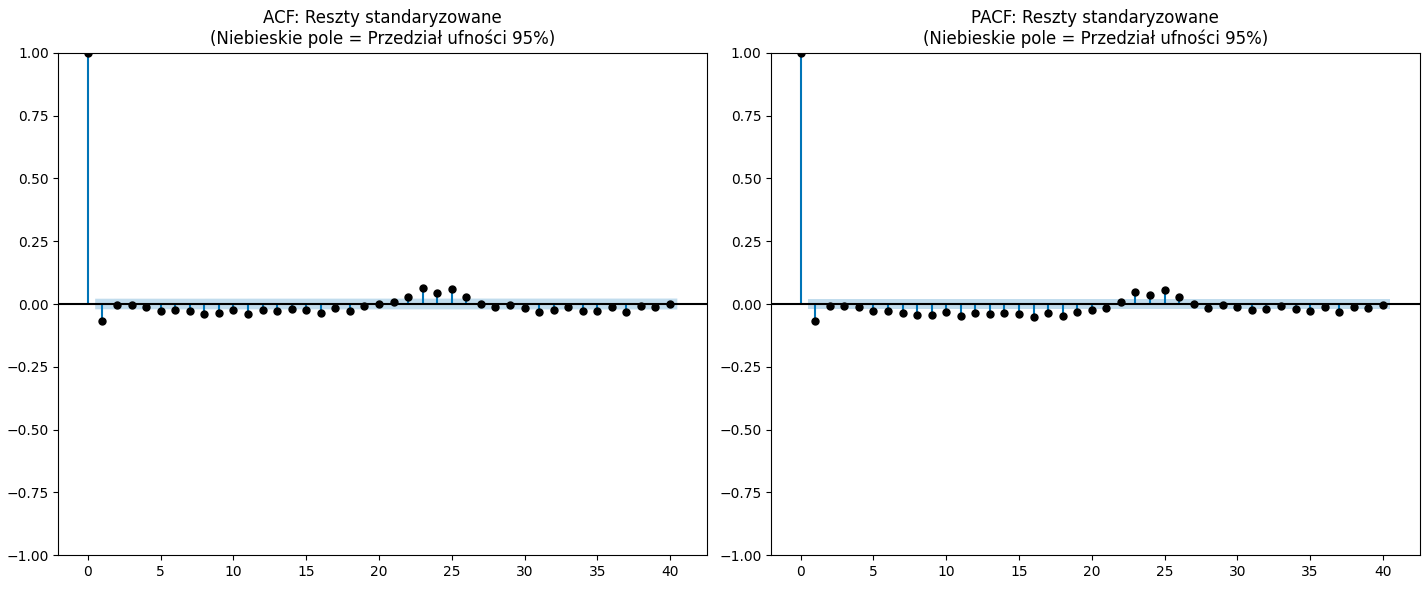
\includegraphics[width=\linewidth]{output12.png}

  \vspace{0.5em} % odstęp między obrazkiem a podpisem

  {\small \textbf{Rysunek 10.} Wykres funkcji autokorelacji (ACF) oraz autokorelacji cząstkowej (PACF) standaryzowanych reszt modelu}
\end{center}

Analiza wykresów funkcji autokorelacji (ACF) oraz autokorelacji cząstkowej (PACF) dla reszt standaryzowanych modelu pozwala na sformułowanie następujących wniosków.
Na wykresach ACF/PACF można zaobserwować pojedyncze opóźnienia (lagi), które przekraczają granice 95-procentowego przedziału ufności. Sugeruje to, że model ARMA(3,1) nie wyeliminował całkowicie zależności liniowych z szeregu. W przypadku danych o smogu może to wynikać z silnej sezonowości dobowej (cykl 24h), której prosty model ARMA nie zawsze jest w stanie w pełni "domknąć". Choć proces resztowy zbliżył się do szumu białego, występowanie istotnych statystycznie słupków świadczy o tym, że w błędach prognozy wciąż kryje się pewna, trudna do uchwycenia informacja. Dla danych o wysokiej częstotliwości (godzinowych) dopuszcza się jednak drobne odstępstwa, jeśli model poprawnie oszacował ogólną zmienność (GARCH). Fakt, że większość słupków mieści się w przedziale, potwierdza, że model GARCH(1,1) poradził sobie z redukcją skupisk zmienności, choć nie usunął wszystkich mikro-zależności.

\subsection{Porównanie linii kwantylowych z trajektorią}
Kluczowym etapem oceny jakości dopasowania modelu jest sprawdzenie, czy wyestymowane parametry pozwalają na wygenerowanie procesów o właściwościach statystycznych zgodnych z danymi empirycznymi. W tym celu przeprowadzimy symulację metodą Monte Carlo, generując $N=1000$ niezależnych trajektorii na podstawie modelu ARMA(3,1)+GARCH(1,1) z rozkładem t-Studenta.
Na podstawie uzyskanych symulacji wyznaczono linie kwantylowe (rzędu $5\%$, $50\%$ oraz $95\%$), które definiują obszar, w jakim z wysokim prawdopodobieństwem powinny zawierać się realizacje procesu. \\
{
\begin{center}
  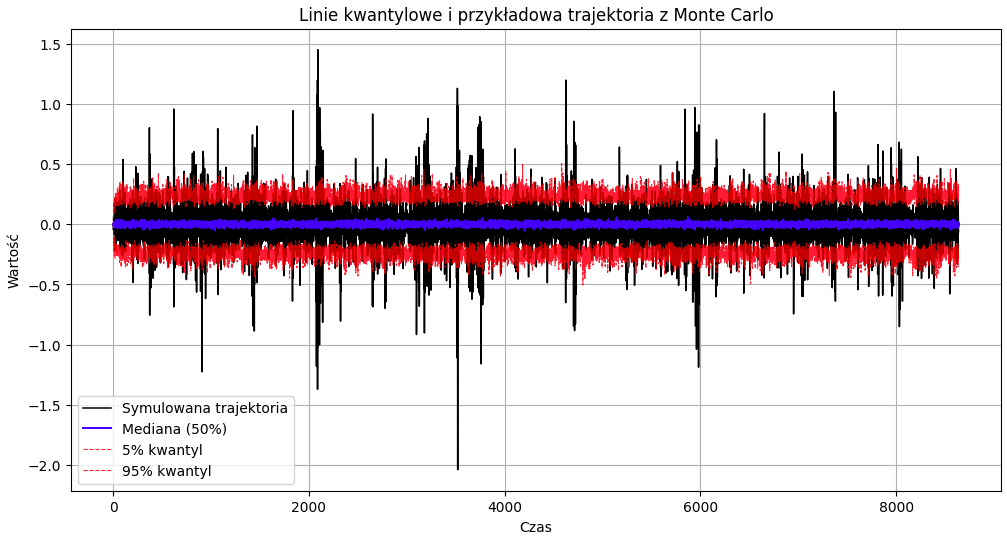
\includegraphics[width=\linewidth]{output10.png}

  \vspace{0.5em} % odstęp między obrazkiem a podpisem

  {\small \textbf{Rysunek 11.} Analiza rozkładu trajektorii modelu: porównanie pojedynczej symulacji z pasmem ufności wyznaczonym przez kwantyle $5\%$ i $95\%$}
\end{center}

Trajektoria symulowana na podstawie parametrów ARMA(3, 1)+GARCH(1,1) wizualnie przypomina rzeczywiste dane stężeń PM2.5, co świadczy o bardzo dobrym dopasowaniu modelu. Model poprawnie odtwarza zmienność, którą obserwujemy w pomiarach we Wrocławiu. Wyznaczone linie kwantylowe tworzą tzw. „korytarz ufności” dla przyszłych realizacji procesu. Szerokość tego korytarza nie jest stała w czasie, co pozwala modelowi na elastyczne reagowanie na okresy zwiększonej niestabilności powietrza.
Gdyby zastosowano rozkład normalny, korytarz kwantylowy byłby znacznie węższy, a wiele realizacji „wypadałoby” poza jego granice. Dzięki zastosowaniu parametru $\nu \approx 6$ (rozkład t-Studenta), linie kwantylowe poprawnie obejmują gwałtowne skoki (tzw. gruby ogon rozkładu), co czyni model użytecznym w systemach wczesnego ostrzegania przed smogiem. Skupienie mediany $50\%$ wokół zera potwierdza, że proces (po zastosowaniu różnicowania) jest stacjonarny i nie wykazuje tendencji do „uciekania” w nieskończoność. Oznacza to, że model jest stabilny numerycznie i nadaje się do prognozowania krótko- i średnioterminowego.

\subsection{Prognoza dla przyszłych obserwacji i porównanie z rzeczywistymi danymi.}
Ostatnim etapem oceny dopasowania modelu ARMA-GARCH jest sprawdzenie jego zdolności do prognozowania przyszłych wartości, które nie były wykorzystane w procesie estymacji parametrów (tzw. próba testowa). Pozwala to ocenić, jak model zachowuje się w starciu z "nowymi" danymi i czy wyznaczone teoretycznie przedziały ufności pokrywają rzeczywistą trajektorię zmian stężeń PM2.5.\\
W niniejszej analizie przyjmujemy horyzont prognozy $h = 24$ godziny. Zbiór danych został podzielony w taki sposób, aby model "nauczył się" dynamiki szeregu na danych historycznych, a następnie wygenerował przewidywania dla ostatniej doby zarejestrowanej w pliku wynikowym.\\
Głównym celem tego etapu nie jest jedynie trafienie w punktową wartość stężenia pyłów, lecz weryfikacja, czy model poprawnie szacuje obszar ryzyka. Ponieważ szereg czasowy PM2.5 charakteryzuje się dużą losowością i zmiennością uwarunkowaną meteorologicznie, kluczowym wskaźnikiem jakości modelu jest utrzymanie się rzeczywistych obserwacji wewnątrz pasma ufności wyznaczonego przez warunkową wariancję (GARCH).

\begin{center}
  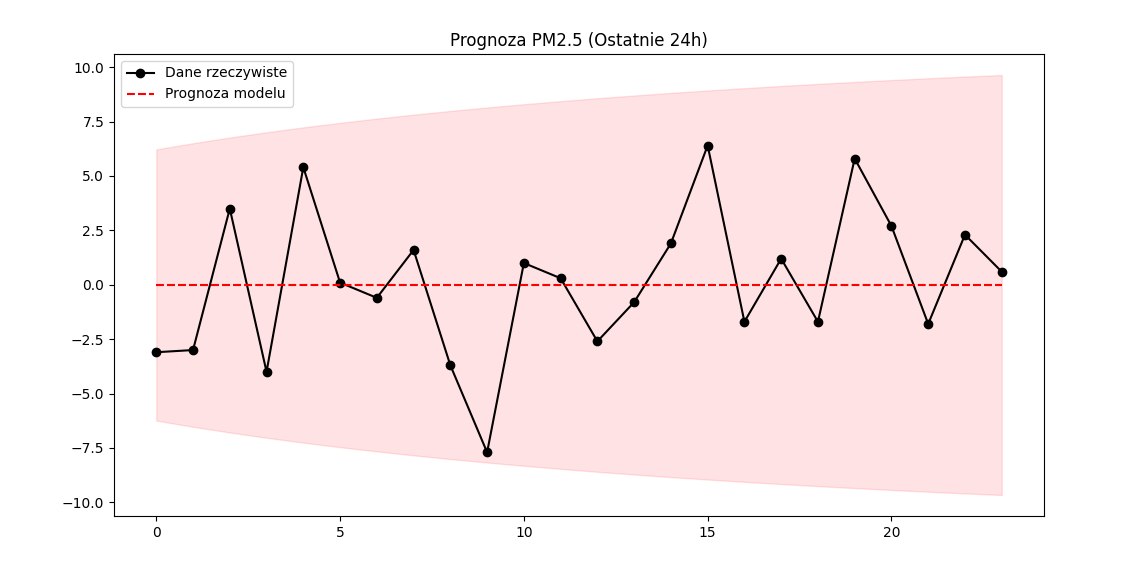
\includegraphics[width=\linewidth]{output13.png}

  \vspace{0.5em} % odstęp między obrazkiem a podpisem

  {\small \textbf{Rysunek 12.} Porównanie prognozy modelu ze stanem faktycznym dla stężeń PM2.5 w ciągu ostatnich 24 godzin wraz z przedziałem ufności}
\end{center}

Prognoza średniej na poziomie bliskim zeru wskazuje na brak silnego trendu kierunkowego w badanym oknie czasowym i tendencję procesu do powrotu do średniej (mean reversion).\\
Fakt, że rzeczywiste zmiany stężeń PM2.5 (czarna linia) oscylują w granicach wyznaczonego przedziału ufności, potwierdza, że model poprawnie zidentyfikował parametry zmienności badanego zjawiska.\\
Model ARMA-GARCH nie służy do precyzyjnego przewidywania momentu „skoku” stężenia, ale do określenia bezpiecznych granic, w jakich te skoki mogą się odbywać. Pod tym względem model jest dopasowany prawidłowo, gdyż rzeczywistość nie „zaskoczyła” modelu wyjściem poza pas ufności.

\section{Weryfikacja założeń dotyczących szumu}
Aby uznać reszty w modelu jako szum losowy, muszą one spełniać poniższe założenia: 
\begin{itemize}
    \item Średnia reszt $E (\epsilon_t) = 0$.
    \item Wariancja $Var (\epsilon_t) = \sigma^2$ jest niezmienna w czasie.
    \item Reszty są niezależne od wcześniejszych wartości szeregu oraz wcześniejszych szumów.
    \item W klasycznym modelu reszty mają rozkład normalny, jednak w naszym przypadku będzie to rozkład Skewed-t. 
\end{itemize}

\subsection{Średnia}
Zaczniemy od wykresu standaryzowanych reszt. Normalizujemy reszty, aby przekształcić je do postaci bezjednostkowej i uniezależnić od wariancji szumu. \\

\begin{center}
  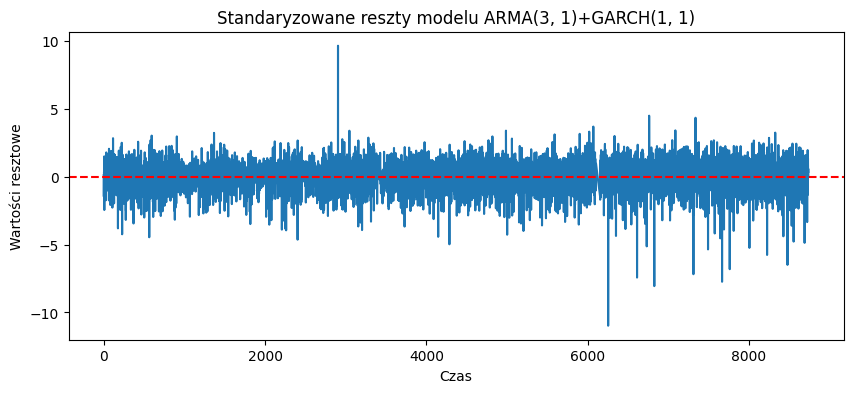
\includegraphics[width=\linewidth]{outp5.png}

  \vspace{0.5em} % odstęp między obrazkiem a podpisem

  {\small \textbf{Rysunek 13.} Wykres wartości resztowych}
\end{center}

Z wykresu można wywnioskować, że wartości resztowe oscylują wokół średniej zero. Dodatkowo, mediana reszt dla tej trajektorii modelu wynosi \fbox{$\tilde{e} = 0.0494$}. Jednak, żeby kompleksowo udowodnić, że średnia reszt jest równa zero, wykonamy test t-Studenta. 

\paragraph{Teoria} 
Test t pozwala zweryfikować, czy średnia w populacji jest równa określonej wartości \(\mu_0\), na podstawie danych z próby o średniej \(\bar{x}\) i odchyleniu standardowym \(s\).

\[
\begin{cases}
H_0: \mu = \mu_0  \\
H_1: \mu \neq \mu_0 \\
\end{cases}
\]

Możliwe są też hipotezy jednostronne, np. \(H_1: \mu > \mu_0\) lub \(H_1: \mu < \mu_0\).

Statystyka testowa \(t\) jest obliczana według wzoru:

\[
t = \frac{\bar{x} - \mu_0}{s / \sqrt{n}},
\]

gdzie:

\begin{itemize}
    \item \(\bar{x}\) — średnia z próby,
    \item \(\mu_0\) — wartość średniej pod hipotezą zerową,
    \item \(s\) — odchylenie standardowe z próby,
    \item \(n\) — liczebność próby.
\end{itemize}

Statystyka \(t\) ma rozkład t-Studenta ze stopniami swobody \(df = n - 1\). \\
\paragraph{Wyniki modelu}
Dla naszych danych przeprowadziliśmy test t, z następującymi hipotezami: \\
\[
\begin{cases}
H_0: \mu = 0  \\
H_1: \mu \neq 0 \\
\end{cases}
\]

\begin{table}[h]
\centering
    \caption{Test t dla poziomu istotności $\alpha = 0.05$}
    \begin{tabular}{|c|c|}
    \hline
    P-wartość & $0.1182$ \\
    \hline
    Wartość statystyki testowej t & $-1.5625$ \\
    \hline
    \end{tabular}
\end{table} 

Różnica od wartości hipotezy zerowej - zero - nie jest statystycznie istotna. Patrząc na wartość statystyki testowej t, istnieje brak podstaw do odrzucenia hipotezy zerowej, która zakłada średnią zero. 

\subsection{Wariancja}
W celu diagnostyki wariancji reszt z modelu ARMA(3,1)+GARCH(1,1) zastosowaliśmy centrowanie wokół zera oraz odrzucenie 1$\%$ skrajnych wartości. 

\paragraph{Teoria}
\ding{172} Centrowanie reszt polega na odjęciu średniej od każdej wartości reszty modelu, co daje reszty o średniej równej zero. Formalnie, dla reszt \( e_i \) z próby o rozmiarze \( n \):

\[
\tilde{e}_i = e_i - \bar{e}, \quad \text{gdzie} \quad \bar{e} = \frac{1}{n} \sum_{i=1}^n e_i.
\]

Centrowanie reszt jest ważne, ponieważ wiele metod statystycznych zakłada, że reszty mają średnią zero, co wpływa na poprawność estymacji i interpretacji modelu.

\ding{173} Winsorowanie to technika ograniczania wpływu wartości odstających poprzez zastąpienie skrajnych obserwacji wartościami bliższymi centrum rozkładu. 

Formalnie, dla zbioru danych \( \{x_1, x_2, \dots, x_n\} \), winsorowana wartość \( x_i^* \) na poziomie $p\%$ to:

\[
x_i^* = 
\begin{cases}
Q_{p}, & x_i < Q_{p}, \\
x_i, & Q_{p} \leq x_i \leq Q_{1-p}, \\
Q_{1-p}, & x_i > Q_{1-p},
\end{cases}
\]

gdzie \( Q_{p} \) oznacza \( p \)-ty percentyl danych.

Winsorowanie pomaga zmniejszyć wpływ ekstremalnych wartości na estymacje statystyczne, poprawiając stabilność i odporność analiz.

\paragraph{Wyniki modelu}
Centrowanie usuwa drobny przesunięty trend średniej, a winsoryzacja ogranicza wpływ ekstremów na testy statystyczne, nie zmieniając zasadniczej struktury reszt. Procedury te pozwalają w wiarygodny sposób sprawdzić, czy reszty zachowują się jak biały szum – w kontekście stałej wariancji. \\
W przypadku winsorowania na wybranym przez nas poziomie 1\% obserwacje poniżej 1. percentyla są zastępowane wartością 1. percentyla, a obserwacje powyżej 99. percentyla są zastępowane wartością 99. percentyla. \\

\begin{center}
  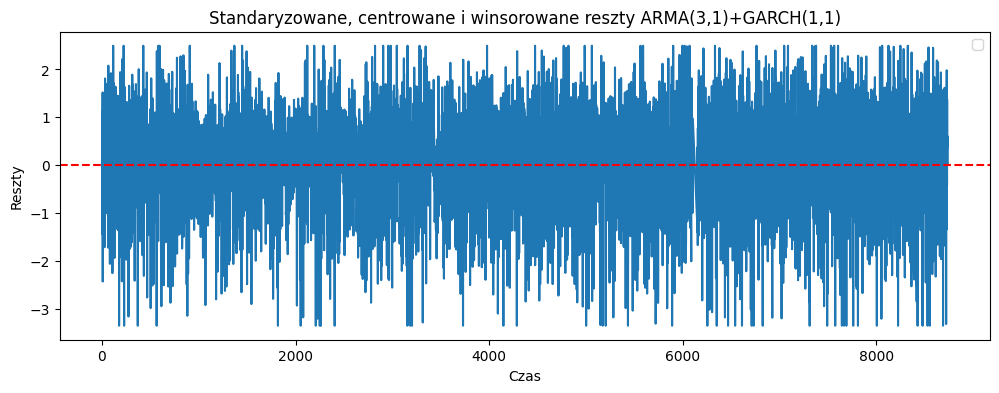
\includegraphics[width=\linewidth]{out6.png}

  \vspace{0.5em} % odstęp między obrazkiem a podpisem

  {\small \textbf{Rysunek 14.} Oczyszczone wartości resztowe}
\end{center}

Amplituda fluktuacji jest dosyć jednorodna oraz nie widać długich okresów podwyższonej zmienności. Wizualna analiza standaryzowanych reszt nie wskazuje na występowanie klastrów zmienności, co sugeruje skuteczną stabilizację wariancji przez model GARCH(1,1). Przejdziemy teraz do testów statystycznych. 

\paragraph{Teoria}
\ding{172} Test ARCH-LM służy do wykrywania efektu autoregresyjnej heteroskedastyczności (ARCH) w resztach modelu.  
Hipotezy testu:
\[
\begin{cases}
H_0: \text{brak efektu ARCH (brak zależności wariancji od przeszłych reszt)} \\
H_1: \text{występuje efekt ARCH}
\end{cases}
\]

Statystyka testowa jest oparta na regresji kwadratów reszt na ich opóźnieniach i ma postać:

\[
LM = n R^2,
\]

gdzie:

\begin{itemize}
    \item \( n \) — liczba obserwacji,
    \item \( R^2 \) — współczynnik determinacji z regresji kwadratów reszt na opóźnieniach.
\end{itemize}

Wartość \(LM\) asymptotycznie ma rozkład chi-kwadrat z \(q\) stopniami swobody, gdzie \(q\) to liczba opóźnień. \\

\ding{173} Test Ljunga-Boxa bada, czy w resztach szeregu czasowego występuje autokorelacja.

Hipotezy testu:

\[
\begin{cases}
H_0: \text{reszty są niezależne (brak autokorelacji)} \\
H_1: \text{reszty są autokorelowane}
\end{cases}
\]

Statystyka testowa jest definiowana jako:

\[
Q = n(n+2) \sum_{k=1}^m \frac{\hat{\rho}_k^2}{n-k},
\]

gdzie:

\begin{itemize}
    \item \( n \) — liczba obserwacji,
    \item \( m \) — liczba opóźnień (lagów) testowanych,
    \item \( \hat{\rho}_k \) — estymator współczynnika autokorelacji rzędu \( k \) reszt.
\end{itemize}

Pod rozkładem \(H_0\), statystyka \(Q\) ma rozkład chi-kwadrat z \(m\) stopniami swobody. \\

\ding{174} Test Ljunga-Boxa można również zastosować do kwadratów reszt, aby wykryć autokorelację wariancji (efekt ARCH).

Hipotezy testu:
\[
\begin{cases}
H_0: \text{kwadraty reszt są niezależne (brak autokorelacji wariancji)} \\
H_1: \text{kwadraty reszt są autokorelowane}
\end{cases}
\]

Statystyka testowa ma tę samą postać co poprzednio, ale dotyczy autokorelacji kwadratów reszt:

\[
Q = n(n+2) \sum_{k=1}^m \frac{\hat{\rho}_{k,\,e^2}^2}{n-k},
\]

gdzie \( \hat{\rho}_{k,\,e^2} \) to estymator współczynnika autokorelacji rzędu \( k \) dla kwadratów reszt. 

\paragraph{Wyniki modelu} 

\begin{center}
\captionof{table}{Testy wartości resztowych, dla poziomu istotności $\alpha = 0.05$}
\begin{tabular}{|c|c|c|}
\hline
\textbf{Statystyka testowa} & \textbf{Wartość statystyki} & \textbf{P-wartość statystyki} \\
\hline
ARCH-LM & 79.82 & 0.00 \\
Ljunga-Boxa dla reszt (lag = 10) &  54.64 & $3.69 \cdot 10^{-8}$ \\
Ljunga-Boxa dla kwadratów reszt (lag = 10) & 84.11 & $7.83 \cdot 10^{-14}$ \\
\hline
\end{tabular}
\end{center}

Testy ARCH-LM oraz Ljunga–Boxa dla kwadratów reszt wskazują na statystycznie istotne zależności, jednak ich skala oraz brak wyraźnych klastrów zmienności w analizie wizualnej sugerują, że model skutecznie redukuje dominującą część heteroskedastyczności. \\

Model GARCH nie zakłada stałej bezwarunkowej wariancji procesu, lecz modeluje jej zmienność warunkową. Celem standaryzacji reszt jest uzyskanie procesu o ustabilizowanej wariancji w sensie praktycznym, a nie spełnienie klasycznego założenia homoskedastyczności. \\

Pomimo skutecznego usunięcia zależności w średniej, reszty modelu wykazują pozostałą zależność w wariancji, co oznacza, że nie spełniają one ścisłych założeń białego szumu. To zjawisko jest jednak typowe dla danych środowiskowych o wysokiej częstotliwości czasowej, w których zmienność może być determinowana przez nieobserwowane czynniki meteorologiczne oraz cykle dobowe i sezonowe. Zatem wskazuje to raczej na ograniczenia prostej specyfikacji GARCH(1,1) niż na fundamentalną niepoprawność modelu. \\

\subsection{Niezależność}

\begin{center}
  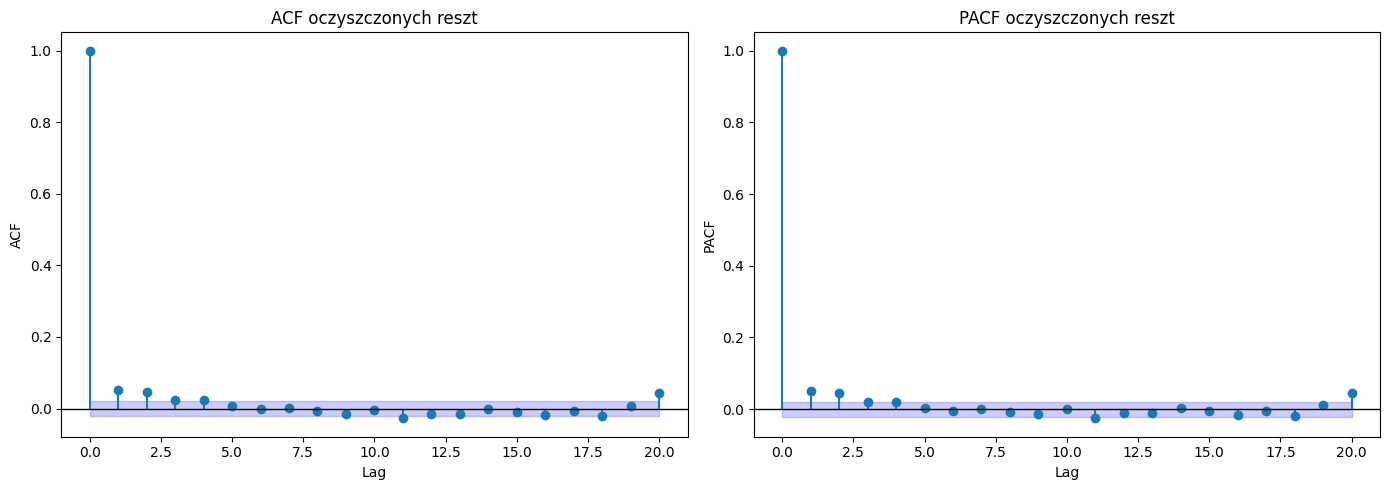
\includegraphics[width=\linewidth]{out7.png}

  \vspace{0.5em} % odstęp między obrazkiem a podpisem

  {\small \textbf{Rysunek 15.} Funkcja autokowariancji oraz częściowej autokowariancji}
\end{center}

Poza pierwszym lagiem, żaden pojedyczny lag nie wychodzi poza wyraźnie poza przedziały ufności. Autokorelacje są bardzo małe, oscylują wokół zera. Wizualnie istnieje brak istotnej autokorelacji. \\

Patrząc na wynik statystyki testowej testu Ljunga-Boxa z poprzedniej sekcji, widzimy że hipoteza o niezależności jest odrzucona. Jednak są funkcje autokowariancji oraz testy Ljunga-Boxa badają różne aspekty statystyczne. Ljung-Box testuje hipotezę globalną, a ACF i PACF hipotezę lokalną. \\

Wnioskując z obydwóch wyników możemy powiedzieć, że jest brak istotnych pojedynczych lagów oraz wyraźnych autokorelacji na wykresach ACF i PACF. Za to test Ljunga–Boxa wskazuje że istnieje istotna suma słabych zależności. Rozbieżność ta wynika z dużej liczby obserwacji, przy której test charakteryzuje się wysoką mocą i wykrywa wiele bardzo słabych zależności niewidocznych w analizie wizualnej. \\

\subsection{Rozkład reszt}

\begin{center}
  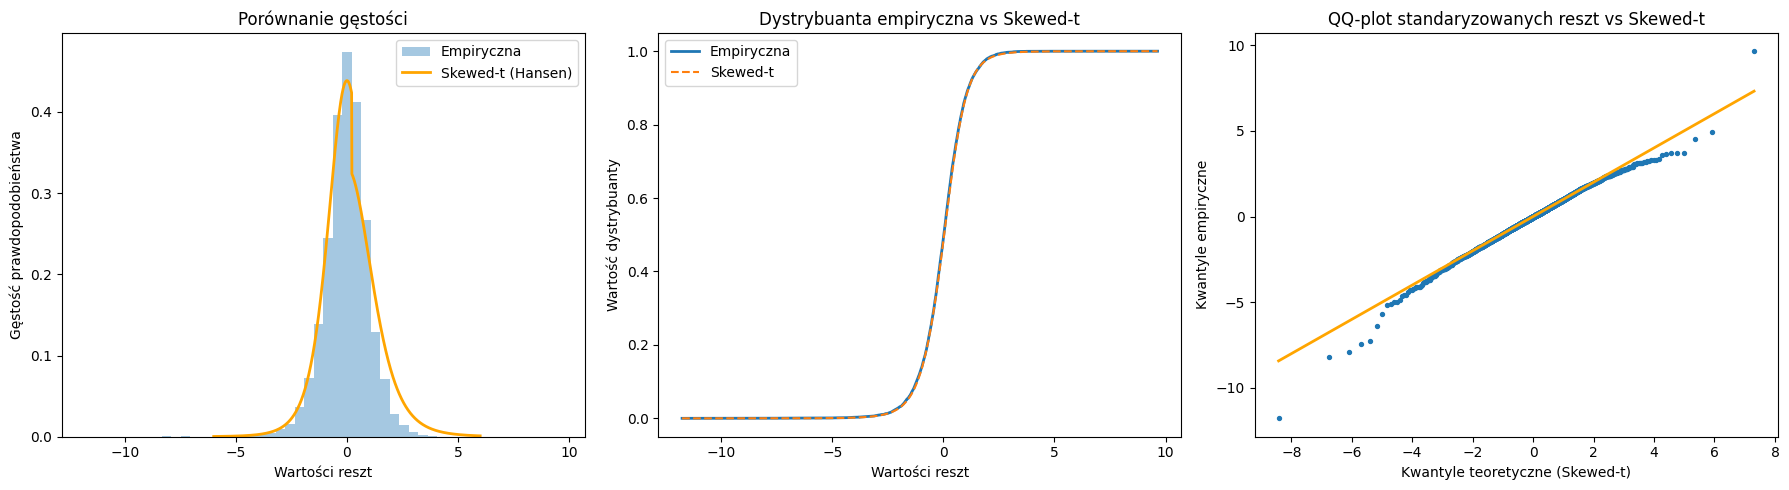
\includegraphics[width=\linewidth]{skew.png}

  \vspace{0.5em} % odstęp między obrazkiem a podpisem

  {\small \textbf{Rysunek 16.} Porównanie rozkładu reszt z rozkładem Skewed-t}
\end{center}

\paragraph{Teoria}
\ding{172} Rozkład Skewed-t, zaproponowany przez Hansa Hansaena, jest rozszerzeniem klasycznego rozkładu t-Studenta o dodatkowy parametr skośności, co pozwala na modelowanie asymetrycznych rozkładów z ciężkimi ogonami.  \\

Dla zmiennej losowej \(X\) o rozkładzie Skewed-t z parametrami \(\nu > 2\) (stopnie swobody) oraz \(\lambda \in (-1,1)\) (skośność), gęstość jest definiowana przez:

\[
f(x; \nu, \lambda) = 
\begin{cases}
\frac{1 - \lambda}{1 + \lambda} \, t_{\nu}\left( \frac{1 - \lambda}{1 + \lambda} x \right), & x < -\frac{a}{c}, \\[10pt]
\frac{1 + \lambda}{1 - \lambda} \, t_{\nu}\left( \frac{1 + \lambda}{1 - \lambda} x \right), & x \geq -\frac{a}{c},
\end{cases}
\]

gdzie \(t_{\nu}(\cdot)\) to gęstość rozkładu t-Studenta o \(\nu\) stopniach swobody, a \(a, c\) to funkcje parametrów \(\nu, \lambda\) określone wzorami:

\[
a = \frac{4 \lambda (\nu - 2)}{(\nu - 1) \sqrt{1 + 3 \lambda^2}}, \quad
c = \sqrt{1 + 3 \lambda^2 - a^2}.
\]

\ding{173} Test Kołmogorowa-Smirnowa (KS) służy do porównania rozkładu empirycznego próbki z rozkładem teoretycznym. Niech \( F(x) \) będzie dystrybuantą rozkładu teoretycznego, a \( F_n(x) \) dystrybuantą empiryczną próby o rozmiarze \( n \).

Statystyka testowa jest zdefiniowana jako:

\[
D_n = \sup_x \left| F_n(x) - F(x) \right|
\]

gdzie \( \sup_x \) oznacza supremum różnicy pomiędzy dystrybuantami.

Im mniejsza wartość \( D_n \), tym lepsze dopasowanie rozkładu teoretycznego do danych. \\

\ding{174} Test Andersona-Darlinga (AD) jest modyfikacją testu KS, która kładzie większy nacisk na dopasowanie rozkładu w ogonach rozkładu. \\

Niech \( X_{(1)} \leq X_{(2)} \leq \dots \leq X_{(n)} \) będą uporządkowanymi obserwacjami z próby, a \( F \) dystrybuantą rozkładu teoretycznego. \\ 

Statystyka testowa jest dana wzorem:
\[
A^2 = -n - \frac{1}{n} \sum_{i=1}^n \left[ (2i - 1) \left( \ln F(X_{(i)}) + \ln \left( 1 - F(X_{(n+1-i)}) \right) \right) \right]
\]
Większe wartości \( A^2 \) wskazują na większe odchylenia od rozkładu teoretycznego.

\paragraph{Wyniki modelu}
Dla naszego modelu mamy parametry: 
\begin{table}[h]
    \centering
    \caption{Parametry rozkładu}
    \begin{tabular}{|c|c|}
    \hline
    \textbf{Parametr} & \textbf{Wartość} \\
    \hline
    Stopnie swobody & 5.38 \\
    Skośność & -0.07 \\
    \hline
    \end{tabular}
\end{table} \\
Dzięki tym wartościom wiemy, że rozkład reszt wybranego modelu ma grube ogony. Za to $\lambda = -0.07$, która jest parametrem skośności (czy też asymetrii), jako że jest ujemna, sugeruje nam że rozkład jest przesunięty w lewo - ma dłuższy ogon po lewej stronie. To się potwierdza na wykresach. \\

Pomimo symetrycznego rozkładu t-Studenta w modelu generującym dane, empiryczny rozkład standaryzowanych reszt wykazuje niewielką asymetrię. W próbie skończonej oraz przy estymowanej wariancji warunkowej rozkład skewed-t zapewnia lepsze dopasowanie, przy czym estymowany parametr skośności jest bliski zeru. \\

Rozkład Skewed-t Hansen pozwala na modelowanie asymetrii i ciężkich ogonów w danych. Po pokazaniu na wykresach porównania rozkładu teoretycznego oraz empirycznych reszt modelu, widzimy że: 
\begin{itemize}
    \item Krzywa gęstości rozkładu Skewed-t dobrze przylega do histogramu empirycznego 
    \item Linia przerywana Skewed-t niemal pokrywa się z empiryczną dystrybuantą
    \item Punkty empiryczne leżą blisko linii Skewed-t
\end{itemize}

\begin{table}[h]
    \centering
    \caption{Testy statystyczne rozkładu, dla poziomu istotności $\alpha = 0.05$}
    \begin{tabular}{|c|c|c|}
    \hline
    \textbf{Test} & \textbf{Wartość statystyki} & \textbf{P-wartość statystyki}\\
    \hline
    Kołmogorowa-Smirnowa & 0.0131 & 0.1034 \\
    Andersona-Darlinga & 1.9445 & 0.0919 \\
    \hline
    \end{tabular}
\end{table} 

Test KS wskazuje na to, że na poziomie istotności $\alpha = 0.05$ nie odrzucamy hipotezy o zgodności rozkładu reszt z rozkładem Skewed-t. Podobnie, test AD również nie daje podstaw do odrzucenia hipotezy zerowej. Różnice na wykresach są subtelne, testy statystyczne nie odrzucają hipotezy o rozkładzie Skewed-t, zatem przyjmujemy że reszty w naszym modelu są istotnie z rozkładu Skewed-t. 

\section{Zakończenie}
\subsection{Podsumowanie pracy}
W ramach pracy przeprowadzono kompleksową analizę statystyczną stężeń pyłu zawieszonego PM2.5 we Wrocławiu. Proces badawczy obejmował:
\begin{itemize}
    \item transformację szeregu do postaci stacjonarnej (przyrosty godzinowe), co pozwoliło na usunięcie trendów i skupienie się na dynamice zmian,
    \item na podstawie funkcji ACF i PACF oraz kryteriów informacyjnych dobrano model ARMA-GARCH, który najlepiej opisywał występujące w danych zjawisko grupowania zmienności,    \item testy statystyczne potwierdziły, że model poprawnie wyeliminował autokorelację, a reszty mają charakter białego szumu, co świadczy o wysokiej jakości dopasowania.
\end{itemize}

\subsection{Wnioski końcowe}
Głównym wnioskiem płynącym z przeprowadzonej prognozy jest wysoka przydatność modelu klasy GARCH do szacowania ryzyka nagłych zmian jakości powietrza. Choć prognoza punktowa dąży do średniej (0), to wyznaczone przedziały ufności (linie kwantylowe) skutecznie ograniczają rzeczywiste wahania stężeń. Oznacza to, że model poprawnie "przewiduje niepewność".\\
Analiza wykazała, że stężenia PM2.5 charakteryzują się silną zmiennością warunkową. Skoki zanieczyszczeń nie są zdarzeniami całkowicie izolowanymi – występują w grupach (okresy wysokiej zmienności przeplatają się z okresami spokoju). Model GARCH jest idealnym narzędziem do opisu tej specyfiki, co potwierdziło porównanie trajektorii z liniami kwantylowymi.\\
Zastosowanie modelu ARMA-GARCH w systemach monitoringu miejskiego mogłoby pozwolić na generowanie ostrzeżeń nie tylko o przewidywanym poziomie pyłów, ale przede wszystkim o prawdopodobieństwie wystąpienia ekstremalnych skoków stężeń, które są najbardziej szkodliwe dla zdrowia mieszkańców.\\
Należy zauważyć, że model czysto statystyczny nie uwzględnia dodatkowych zmiennych (np. kierunku wiatru, temperatury czy opadów). Dalsze rozszerzenie modelu o te parametry (model ARMAX-GARCH) mogłoby jeszcze bardziej zawęzić przedziały ufności i zwiększyć precyzję prognoz punktowych.

\end{document}